\section{Αξιολόγηση 3D ανακατασκευασμένων μοντέλων}

Στα πλαίσια της αξιολόγησης του πόσο καλά λειτουργεί το δίκτυο ανακατασκευής \enit{3D} επιφανειών με χρήση των βαθιών δικτύων κωδικοποίησης γίνεται λόγος για το πόσο μοιάζει γεωμετρικά το μοντέλο που παράγεται από το δίκτυο σε σχέση με το αντίστοιχο 3D scan του DTU αλλά και η ομοιότητα της σκηνής με την αντίστοιχη φωτογραφία επίβλεψης όταν γίνεται αξιολόγηση και του πεδίου φωτισμού στα πλαίσια της εμφάνισης.  Αλλά, ας ξεκινήσουμε με τις μετρικές αξιολόγησης σε επίπεδο φωτογραφίας.
\section{Μετρικές Αξιολόγησης Αλγορίθμων}
\subsection{PSNR - Λόγος σήματος κορυφής προς θόρυβο}
Για δεδομένη \enit{3D} σκηνή, αυτή της κουκουβάγιας, φαίνεται πως στο παρακάτω διάγραμμα όπου συγκρίνεται η φωτορεαλιστική απόδοση των διαφορετικών αλγορίθμων για πλήθος θέσεων κάμερας δηλαδή όψεων. 
Το PSNR ορίζεται πιο εύκολα μέσω του μέσου τετραγωνικού σφάλματος (MSE). Δεδομένης μιας μονοχρωματικής εικόνας I με μέγεθος m×n και της θορυβώδους προσέγγισής της K, το MSE ορίζεται ως

    \[
    M S E = \frac{1}{mn} \sum_{i=0}^{m-1} \sum_{j=0}^{n-1} [I(i, j) - K(i, j)]^2.
    \]
    
    Το PSNR (σε dB) ορίζεται ως
    
    \[
    P S N R = 10 \cdot \log_{10}\left(\frac{MAXI^2}{MSE}\right) = 20 \cdot \log_{10}\left(\frac{MAXI}{\sqrt{MSE}}\right) = 20 \cdot \log_{10}(MAXI) - 10 \cdot \log_{10}(MSE).
    \]
    
    Εδώ, το MAXI είναι η μέγιστη δυνατή τιμή εικονοστοιχείου της εικόνας. Όταν τα εικονοστοιχεία αναπαρίστανται χρησιμοποιώντας 8 bits ανά δείγμα, αυτή είναι η τιμή 255. Πιο γενικά, όταν τα δείγματα αναπαρίστανται χρησιμοποιώντας γραμμικό PCM με B bits ανά δείγμα, το MAXI είναι $2^{B} - 1$.
\begin{figure}[H]
\centering
      \begin{adjustbox}{width=1\linewidth}
        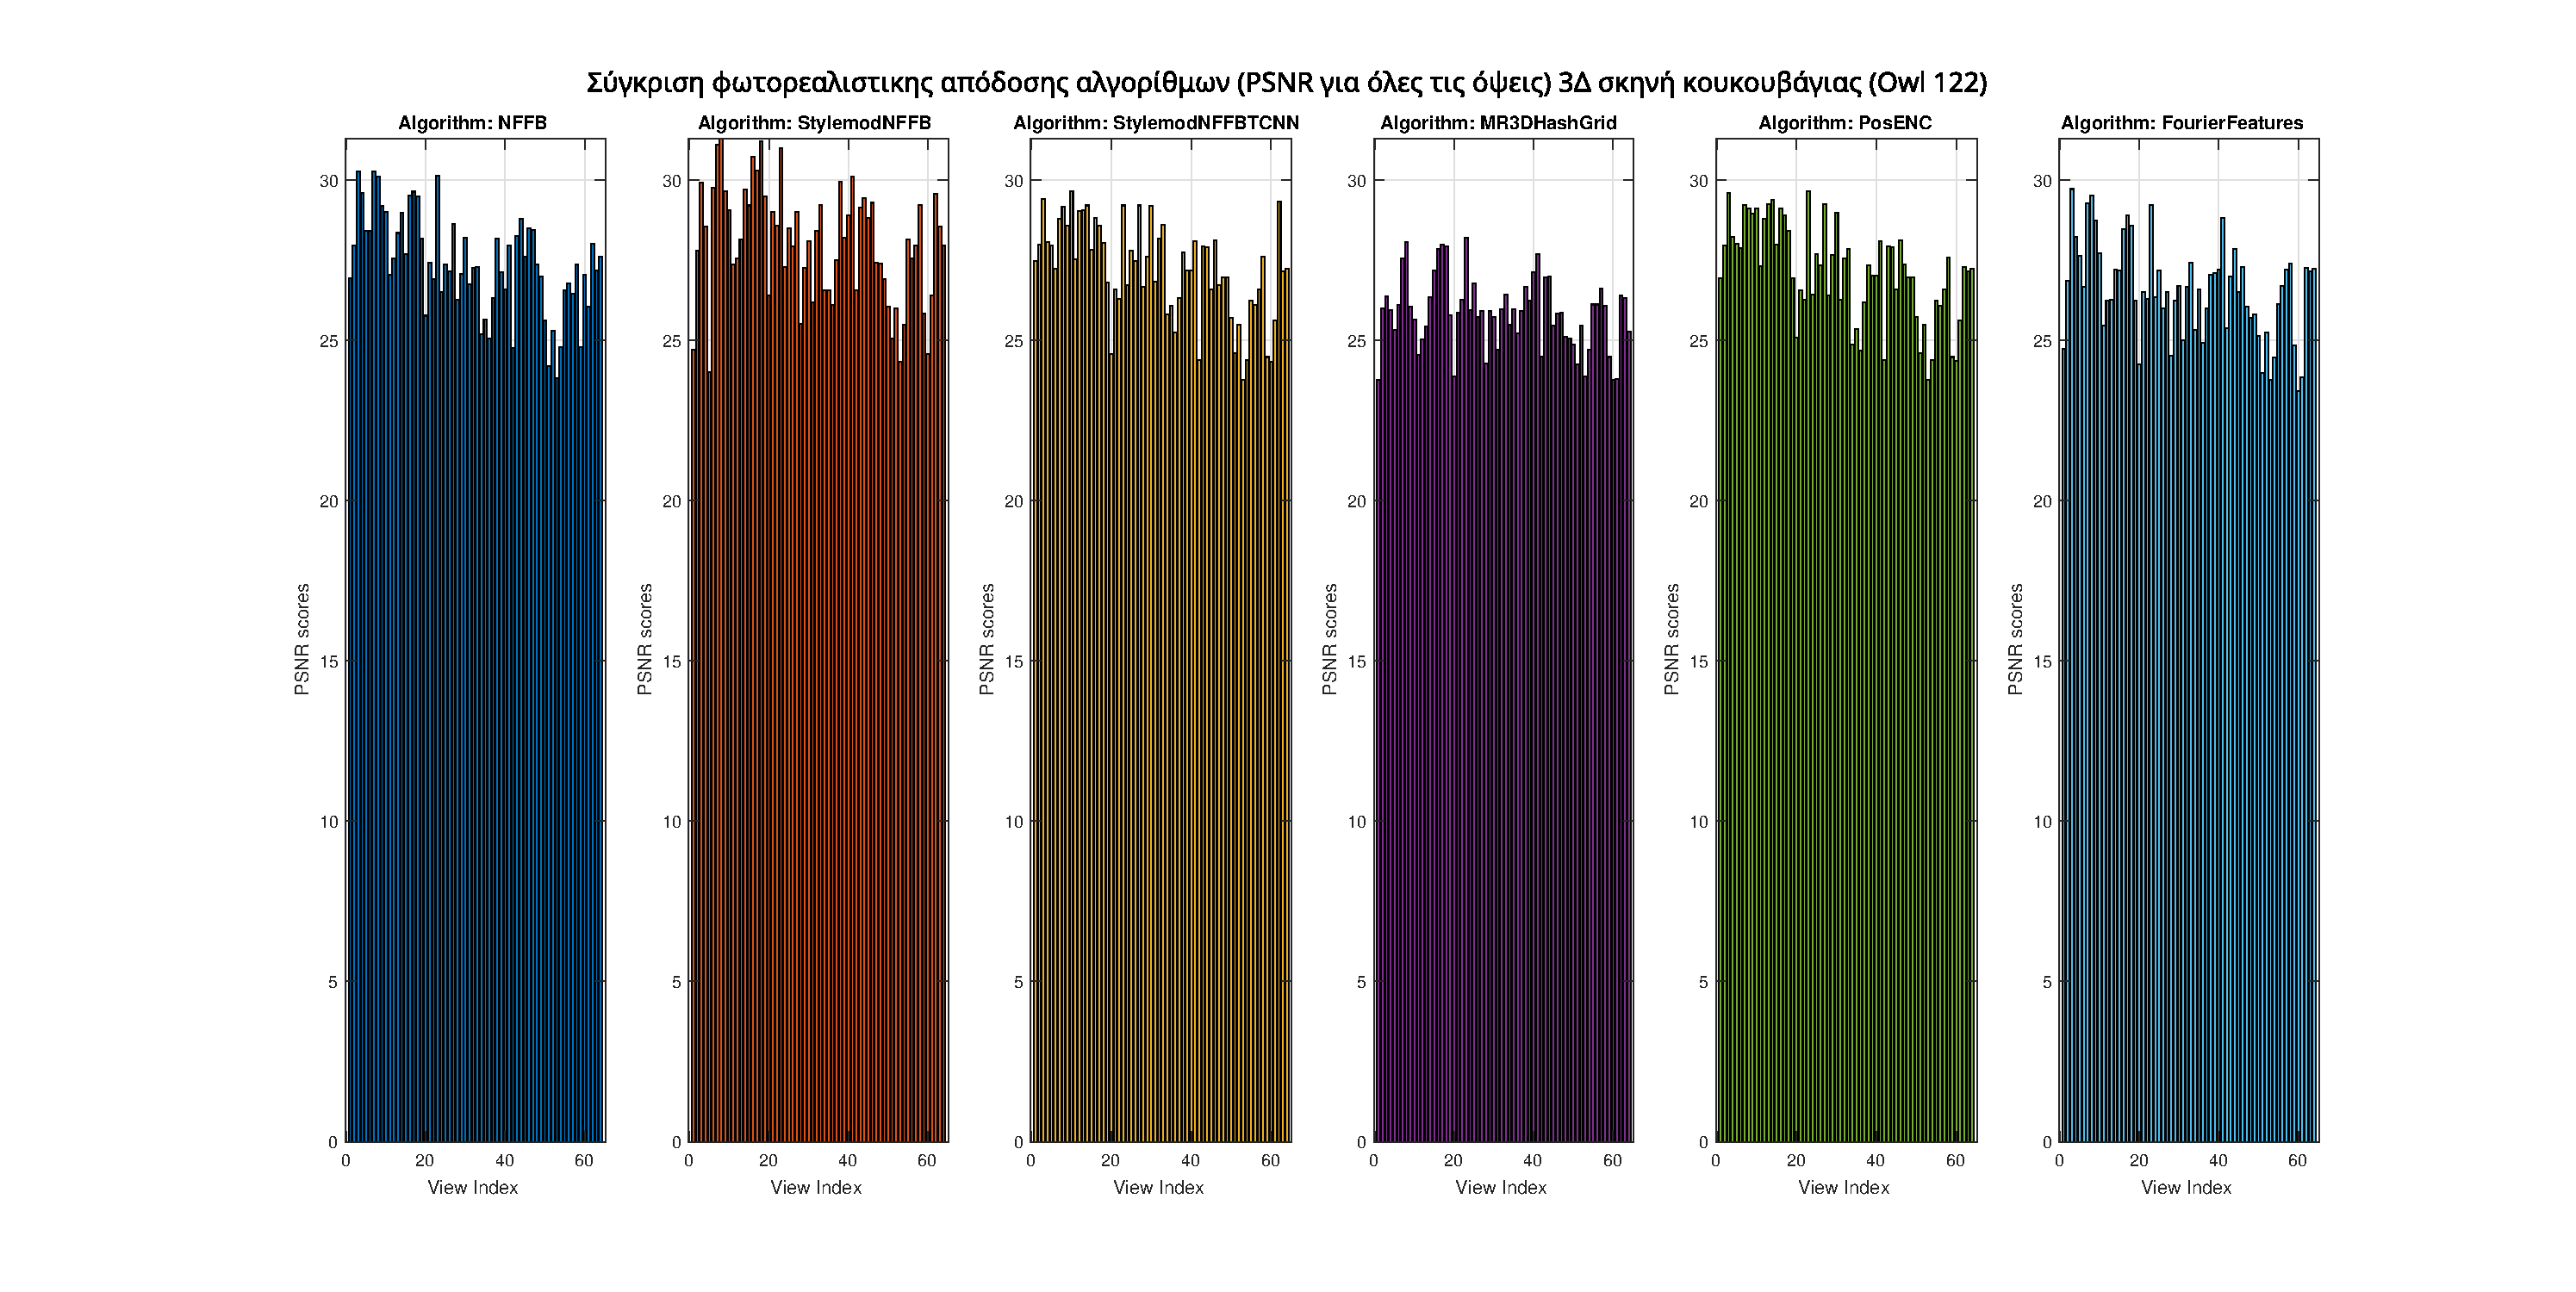
\includegraphics{images/chapter5_img/EvalMetricsPlots/Multiview-MultiAlgorithm-PSNRComparison.eps} % Replace with your figure file
      \end{adjustbox}
    \caption{Σηματοθορυβική σύγκριση αλγορίθμων κωδικοποίησης στην σκηνή της κουκουβάγιας}
    \label{fig:psnrcomparison}
\end{figure}
\par
    Η μετρική PSNR δείχνει πόσο υψηλής ποιότητας είναι η \enit{3D} ανακατασκευή στο επίπεδο της φωτογραφίας του μοντέλου. Μικρές μεταβολές μπορεί να αντιστοιχούν σε πολλαπλάσιο ποσό θορύβου φωτογραφίας μιας και η κλίμακα είναι λογαριθμική. Συγκεκριμένα για 1 μονάδα αύξηση έχουμε 10 φορές λιγότερο θόρυβο. Έτσι αυτό που παρατηρείται στην ανακατασκευή της σκηνής της κουκουβάγιας είναι ότι τα μοντέλα φίλτρων πλεγμάτων Fourier (\enit{Fourier Filter Banks}) είναι σε θέση να μειώσουν το θόρυβο σε όλες τις όψεις αρκετά. Ταυτόχρονα το hashgrid δεν μπορεί να συλλάβει υψηλοσυχνοτικό περιεχόμενο από μόνο του γιατί το πλήθος των επιπέδων ανάλυσης που χρησιμοποιείται είναι μικρό. Ταυτόχρονα η συχνοτική κωδικοποίηση με μπορεί να κάνει καλύτερη δουλειά για λίγα επίπεδα συχνοτήτων αλλά παρουσιάζει μεγάλη διακύμανση στις τιμές και απαιτεί το \enit{Hash Grid Encoding} για εντοπισμό των χαρακτηριστικών περιοχών. Τέλος, τα συγχωνευμένο δίκτυο θυρίδων \enit{(StylemodNFFBTCNN)} φαίνεται να αποτελεί μια ιδανική λύση δεδομένου μικρότερου χρόνου εκπαίδευσης και χρησιμοποιούν την συνδυασμένη μέθοδο των φίλτρων πλεγμάτων Fourier.
\begin{table}[H]
\centering
\begin{tabular}{|l|c|c|c|c|}
\hline
\textbf{PSNR Metric} & \multicolumn{4}{c|}{\textbf{DTU Scenes}} \\
\hline
Embedding Algorithm for IDR Input & \textbf{Owl[122]} & \textbf{Rabbit[110]} & \textbf{Skull[65]} & \textbf{Buda[114]} \\
\hline
Positional Encoding & 27.15 & 22.7 & \textbf{24.58} & \textbf{26.09} \\
\hline
Fourier Features & 26.51 & 22.21 & 22.07 & 23.23 \\
\hline
Multi-Resolution Hash Grid & 25.85 & \textbf{22.73} & 22.74 & 21.81 \\
\hline
Multi-Resolution Hash Grid (\textit{TinyCudaNN}) & 27.26 & 22.33 & & \\
\hline
NFFB & 27.4 & 21.43 & 21.94 & 23.35 \\
\hline
StyleMod NFFB & \textbf{28.04} & 21.97 & 22.96 & 23.96 \\
\hline
StyleModNFFB (\textit{TinyCudaNN}) & 27.57 & 20.57 & 23.48 & 24.55 \\
\hline
\end{tabular}
\caption{Αποτελέσματα αξιολόγησης με τη μετρική PSNR}
\end{table}



\subsection{SSIM(Structure Similarity Index Measure) - Μετρική Δείκτη Δομικής Ομοιότητας Εικόνων}
Η μετρική δείκτη δομικής ομοιότητας (SSIM) είναι μια μέθοδος πρόβλεψης της αντιλαμβανόμενης ποιότητας ψηφιακών τηλεοπτικών και κινηματογραφικών εικόνων, καθώς και άλλων ειδών ψηφιακών εικόνων και βίντεο.Το SSIM είναι ένα μοντέλο βασισμένο στην αντίληψη που θεωρεί την υποβάθμιση της εικόνας ως αντιληπτή μεταβολή της δομικής πληροφορίας, ενώ ενσωματώνει επίσης σημαντικά αντιληπτικά φαινόμενα, συμπεριλαμβανομένων τόσο των όρων κάλυψης φωτεινότητας όσο και των όρων κάλυψης αντίθεσης.Η διαφορά με άλλες τεχνικές όπως το MSE ή το PSNR είναι ότι οι προσεγγίσεις αυτές εκτιμούν τα απόλυτα σφάλματα. Η δομική πληροφορία είναι η ιδέα ότι τα εικονοστοιχεία έχουν ισχυρές αλληλεξαρτήσεις, ιδίως όταν βρίσκονται σε χωρική εγγύτητα.
\begin{table}[H]
\centering
\begin{tabular}{|l|c|c|c|c|}
\hline
\textbf{SSIM Metric} & \multicolumn{4}{c|}{\textbf{DTU Scenes}} \\
\hline
Embedding Algorithm for IDR Input & \textbf{Owl[122]} & \textbf{Rabbit[110]} & \textbf{Skull[65]} & \textbf{Buda[114]} \\
\hline
Positional Encoding & \textbf{0.96} & 0.93 & 0.95 & \textbf{0.91} \\
\hline
Fourier Features & 0.95 & 0.93 & 0.94 & 0.88 \\
\hline
Multi-Resolution Hash Grid & 0.95 & 0.93 & 0.95 & 0.86 \\
\hline
Multi-Resolution Hash Grid (\textit{TinyCudaNN}) & \textbf{0.96} & \textbf{0.94} & & \\
\hline
NFFB & \textbf{0.96} & 0.93 & 0.94 & 0.88 \\
\hline
StyleMod NFFB & \textbf{0.96} & 0.93 & 0.94 & 0.89 \\
\hline
StyleModNFFB (\textit{TinyCudaNN}) & \textbf{0.96} & 0.92 & \textbf{0.96} & 0.88 \\
\hline
\end{tabular}
\caption{Αποτελέσματα αξιολόγησης με τη μετρική SSIM}
\end{table}


\subsection{LPIPS(Learned Perceptual Image Patch Similarity)-  Αντιληπτική Ομοιότητα Μπαλωμάτων Εικόνας σε  μοντέλα αναγνώρισης εικόνας}
Η συγκεκριμένη μετρική είναι μια μέθοδος αξιολόγησης εικόνων που πλέον γίνεται από νευρωνικά δίκτυα. Στην συγκεκριμένη περίπτωση χρησιμοποιείται το Alexnet (προ εκπαιδευμένο μοντέλο αναγνώρισης εικόνας) για να δείξει πόσο διαφέρουν οι εικόνες μεταξύ τους. Όσο μικρότερη είναι η τιμή το LPIPS σημαίνει τόσο κοντά είναι όχι μόνο σε επίπεδο χρώματος(τιμή [r, g, b]) αλλά και σε αυτό που αναπαρίσταται στις δύο εικόνες.
\begin{table}[H]
\centering
\begin{tabular}{|l|c|c|c|c|}
\hline
\textbf{LPIPS Metric} & \multicolumn{4}{c|}{\textbf{DTU Scenes}} \\
\hline
Embedding Algorithm for IDR Input & \textbf{Owl[122]} & \textbf{Rabbit[110]} & \textbf{Skull[65]} & \textbf{Buda[114]} \\
\hline
Positional Encoding & 0.08 & 0.15 & 0.09 & 0.19 \\
\hline
Fourier Features & 0.25 & 0.16 & 0.11 & \textbf{0.10} \\
\hline
Multi-Resolution Hash Grid & 0.08 & 0.14 & 0.1 & 0.19 \\
\hline
Multi-Resolution Hash Grid (\textit{TinyCudaNN}) & \textbf{0.06} & 0.11 & & \\
\hline
NFFB & 0.09 & \textbf{0.03 }& 0.1 & 0.22 \\
\hline
StyleMod NFFB & 0.08 & 0.16 & 0.1 & 0.2 \\
\hline
StyleModNFFB (\textit{TinyCudaNN}) & 0.07 & 0.15 & \textbf{0.08} & 0.16 \\
\hline
\end{tabular}
\caption{Αποτελέσματα αξιολόγησης με τη μετρική LPIPS}
\end{table}

